%
% Portuguese-BR vertion
% 
\documentclass{report}

\usepackage{ipprocess}
% Use longtable if you want big tables to split over multiple pages.
\usepackage{longtable}
\usepackage[utf8]{inputenc} 
\usepackage[brazil]{babel} % Uncomment for portuguese
\usepackage{pdflscape} % set ladscape/portrait pdf pages
\usepackage{tikz}
\usepackage{tikz-uml}
\usepackage{lscape}


\sloppy

\graphicspath{{./pictures/}} % Pictures dir
\makeindex
\begin{document}


%%%%%%%%%%%%%%%%%%%%%%%%%%%%%%%%%%%%%%%%%%%%%%%%%%
%% Building front cover
%%%%%%%%%%%%%%%%%%%%%%%%%%%%%%%%%%%%%%%%%%%%%%%%%%
\DocumentTitle{Documento de Arquitetura}
\Project{Controlador de Estufa.}
\Organization{Universidade Estadual de Feira de Santana}
\Version{Compilação 1.1}
% Make front cover
\capa
%

%%%%%%%%%%%%%%%%%%%%%%%%%%%%%%%%%%%%%%%%%%%%%%%%%%
%% Revision History
%%%%%%%%%%%%%%%%%%%%%%%%%%%%%%%%%%%%%%%%%%%%%%%%%%
\chapter*{Histórico de Revisões}
  \vspace*{1cm}
  \begin{table}[ht]
    \centering
    \begin{tabular}[pos]{|m{2cm} | m{8cm} | m{4cm}|} 
      \hline
      \cellcolor[gray]{0.9}
      \textbf{Date} & \cellcolor[gray]{0.9}\textbf{Descrição} & \cellcolor[gray]{0.9}\textbf{Autor(s)}\\
      \hline
      30/03/2015 &  Desenvolveu a Introdução, Arquitetura do Sistema, Casos de Uso e Esquema Elétrico & Felipe Pinheiro \\ \hline
      30/03/2015 &  Revisão de texto e desenvolvimento da seção Ambiente de Desenvolvimento & Bianca Santana \\ \hline
      31/03/2015 & Revisão do texto de Introdução a seção Visão Geral da Arquitetura & Lucas Almeida \\ \hline 
      31/03/2015 & Seção de Introdução a Visão Geral da Arquitetura & Lucas Almeida \\ \hline 
      xx/xx/xxxx &
      
      \begin{itemize}
        \item Exemplo de;
        \item Revisões em lista;
      \end{itemize}
      & <Autor(es)> \\ \hline 
    \end{tabular}
  \end{table}

% TOC instantiation
\tableofcontents

%%%%%%%%%%%%%%%%%%%%%%%%%%%%%%%%%%%%%%%%%%%%%%%%%%
%% Document main content
%%%%%%%%%%%%%%%%%%%%%%%%%%%%%%%%%%%%%%%%%%%%%%%%%%
\chapter{Introdução}
  
  \section{Propósito do Documento}
      Este documento de arquitetura se baseia em um projeto de controle de um local aberto e uma estufa, onde o usuário poderá solicitar determinadas informações sobre 
      suas condições atuais, além de poder controlar à distância a abertura e fechamento da porta dessa estufa. Aqui serão detalhados todos os requisitos, explicando como 
      eles serão implementados e agrupados ao projeto, dessa forma, definindo a arquitetura do sistema. Os diagramas definidos abaixo, foram baseados em diagramas utilizados
      no campo da Engenharia de Software, devido a semelhança no desenvolvimento de um projeto de Software e de um Sistema Embarcado.

\section{Visão Geral do Documento}
O presente documento é apresentado como segue:
  \begin{itemize}
   \item \textbf{Capítulo 2 --} Este capítulo apresenta uma visão geral da arquitetura, com foco em entrada e saída do sistema e arquitetura geral do mesmo;
   \item \textbf{Capítulo 3 --} Este capítulo descreve a arquitetura interna do IP a partir do detalhamento dos seus componentes, definição de portas de entrada e saída e diagrama de blocos. 
   \item \textbf{Capítulo 4 --} Este capítulo descreve a arquitetura da aplicação Android. 
  \end{itemize}


  % inicio das definições do documento
  \section{Definições}
    \FloatBarrier
    \begin{table}[H]
      \begin{center}
        \begin{tabular}[pos]{|m{5cm} | m{9cm}|} 
          \hline
          \cellcolor[gray]{0.9}\textbf{Termo} & \cellcolor[gray]{0.9}\textbf{Descrição} \\ \hline
          RS232                & Protocolo de comunicação serial utilizado em aplicações que requerem transmissão de dados entre elementos conectados à um mesmo canal. \\ \hline 
          PIC & É um dispositivo caracterizado tipicamente por encapsular um microprocessador, memória de programa e periféricos como: temporizadores, \"watchdog timers\", comunicação 
          serial, conversores Analógico/Digital, geradores de PWM, etc. \\ \hline
          LDR & Dispositivo semicondutor de dois terminais, cuja resistência diminui em função do aumento da intensidade de luz incidente ou vice-versa.\\ \hline
          Sensor de Temperatura & Disposito que permite a monitoração da temperatura ambiente ou da temperatura interna de um sistema eletrônico. \\ \hline 
          USART & É um tipo de periférico de comunicação de dados de forma serial que pode operar de dois modos distintos de funcionamento: síncrono e o assíncrono. \\ \hline
          MAX 232 & É um circuito integrado capaz de converter os sinais de +/- 12 volt (típicos da interface RS232) para sinais 0 à 5 volts compatíveis com as portas do PIC. \\ \hline 
        \end{tabular}
      \end{center}
    \end{table}  
  % fim

  % inicio da tabela de acronimos e abreviacoes do documento
  \section{Acrônimos e Abreviações}
    \FloatBarrier
    \begin{table}[H]
      \begin{center}
        \begin{tabular}[pos]{|m{2cm} | m{12cm}|} 
          \hline
          \cellcolor[gray]{0.9}\textbf{Sigla} & \cellcolor[gray]{0.9}\textbf{Descrição} \\ \hline
          TBD      &  To be defined (A ser definido)  \\ \hline
          LDR & Light Dependent Resistor. (Fotoresistor) \\ \hline 
          LM35 & Sensor de Temperatura \\ \hline
          USART & Universal Synchronous Asynchronous Receiver Trasmitter (Transmissor e Receptor Universal Síncrono e Assíncrono)\\ \hline 
          GPRS & General Packet Radio Service (Serviço de Rádio de Pacote geral) \\ \hline
        \end{tabular}
      \end{center}
    \end{table}  
  % fim

\chapter{Visão Geral da Arquitetura}

  \section{Introdução}
   
      Este capítulo visa apresentar uma visão geral da arquitetura proposta, além das subdivisões das arquitetura em duas esferas: Hardware e Software. Sendo assim, será apresentado 
    nas duas seções: Arquitetura de Hardware e Arquitetura de Software os diagramas de classes de cada módulo e diagramas de bloco com uma visão mais abstrata da arquitetura. A visão 
    mais genérica da arquitetura do sistema é apresentada na seção Descrição Geral da Arquitetura .
    
   \section{Descrição Geral da Arquitetura} 
   
	A partir de uma aplicação para a plataforma Android 2.2, ou superior, o usuário poderá controlar ou visualizar informações de um projeto solarimétrico. Com o aplicativo
	será possível ao usuário solicitar os seguintes dados: temperatura, luminosidade, estado da bateria (“abaixo da metade” ou “acima da metade”). Essas variáveis serão obtidas 
	por meio de sensores, sendo eles: LDR, LM35. Os dados obtidos serão processados por um microcontrolador PIC. 

	A comunicação o módulo de controle da estufa e o usuário será realizada por meio de um módulo GPRS, que permite o envio e o recebimento de mensagem de texto. O interfaceamento 
	do PIC e do módulo GPRS ocorrerá por meio do módulo USART. A troca de informações acontecerá quando o usuário requisitar uma informação ou operação, ou o sistema de controle enviar 
	um dado para o módulo de Software. Solicitada uma informação todas as demais serão enviadas para o usário e junto a elas a data e hora da medição. O sistema a depender da temperatura (caso seja inferior a 20°C
	ou superior a 40°C) aciona ou desliga,automaticamente, o sistema de aquecimento. O usuário também poderá, por motivo de segurança, ligar ou desligar o sistema de aquecimento por meio 
	do aplicativo. 
	
	Quando o sistema for ligado a porta da estufa deve ser fechada automaticamente, e quando desligado a porta deve se abrir. O controle dessa porta será feito com um motor de corrente 
	contínua, onde um circuito de Ponte H controlará a direção de rotação desse motor fazendo com que a porta se movimente. A Figura \ref{figure:arquiteturaGeral} apresenta a visão geral
	do sistema com todos os possíveis módulos e a comunicação entre eles. O Dispositivo Controlador representa o PIC junto com todos os outros dispositivos elétricos necessários para o 
	seu funcionamento.
	
	\begin{figure}[H]
	 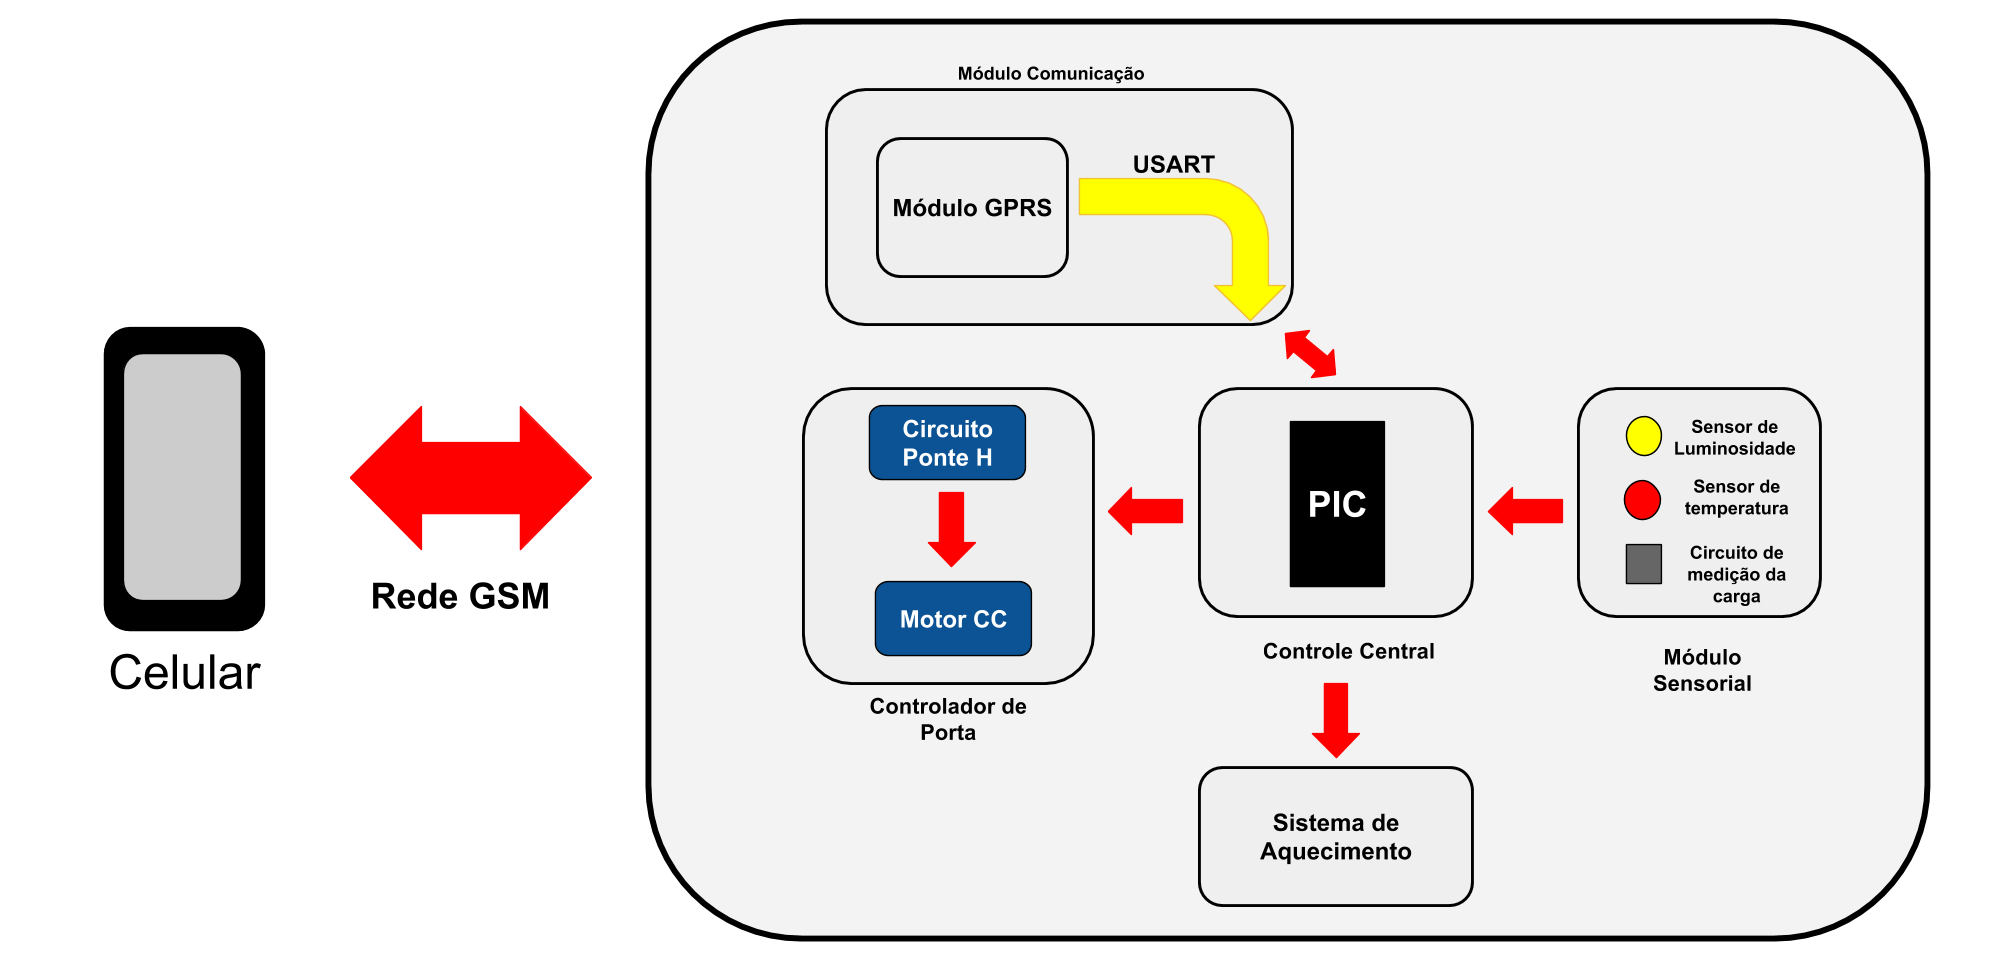
\includegraphics[width=\linewidth]{pictures/visao_geral.png}
	 \caption{Visão abstrata da Arquitetura do Sistema.}
	 \label{figure:arquiteturaGeral}
	\end{figure}

    
    \subsection{Definições dos blocos} \label{defBlocos}
      \FloatBarrier
   
      \begin{longtable}[pos]{| l | m{9cm} |} \hline         
        \multicolumn{1}{|c|}{\cellcolor[gray]{0.9}\textbf{Nome}} & 
        \multicolumn{1}{c|}{\cellcolor[gray]{0.9}\textbf{Descrição}} \\ \hline
        \endfirsthead
        \hline
        \multicolumn{2}{|l|}%
        {{\bfseries continuação da página anterior}} \\
        \hline
        \multicolumn{1}{|c|}{\cellcolor[gray]{0.9}\textbf{Nome}} & 
        \multicolumn{1}{c|}{\cellcolor[gray]{0.9}\textbf{Descrição}} \\ \hline
        \endhead

        \multicolumn{2}{|r|}{{continua na próxima página}} \\ \hline
        \endfoot

        \hline
        \endlastfoot

	 Módulo em Software    &  Aplicação desenvolvida para plataforma Android com versão mínima 2.2    \\ \hline
	 Módulo de Comunicação &  Módulo GPRS responsável por enviar e receber as mensagens de texto    \\ \hline
         Controlador Central      &  Módulo que realiza o controle do sistema de aquecimento e aciona o módulo de 
				  controle da porta a depender das informações recebidas do usário ou lidas dos sensores.  \\ \hline
         Controlador da porta     &  Módulo que contém o circuito Ponte H responsável pelo controle de abrir e fechar a porta da estufa adequadamente\\ \hline
         Sistema de Aquecimento & Sistema independete responsável por aquecer a estufa \\ \hline 
         Módulo Sensorial      &  Módulo que realiza a leitura das informações dos sensores: LDR e LM35, e realiza a leitura do estado da
         bateria a partir de um circuito resistivo\\ 
      \end{longtable}
   
   \section{Diagrama de Atividade}
   
    Na Figura \ref{figure:diagramaXAtividades} e na Figura \ref{figure:diagramaYAtividades} podemos analisar as atividades exercidas pelos módulos da Estufa e de Ambiente Externo respectivamente. 
    As linhas vermelhas representam quebras de fluxo devido à comunicação com módulo móvel. Note também que após uma atividade finalizada 
    odemos redirecionar o fluxo, inclusive para o inicio da mesma atividade.
    
      \begin{figure}[H]
	 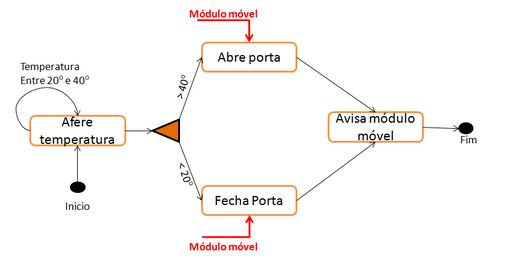
\includegraphics[width=\linewidth]{pictures/diagramaXAtividades.JPG}
	 \caption{Diagrama de Atividade da Estufa.}
	 \label{figure:diagramaXAtividades}
	\end{figure}
	
      \begin{figure}[H]
	 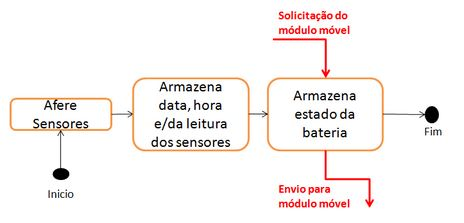
\includegraphics[width=\linewidth]{pictures/diagramaYAtividades.JPG}
	 \caption{Diagrama de Atividade da Estufa.}
	 \label{figure:diagramaYAtividades}
	\end{figure}
	

   \section{Diagrama de Sequência}
   
   Esta Seção tem como objetivo apresentar os principais Diagramas de Atividade. As Figuras \ref{figure:ativar_sistema_aquecimento} e
   \ref{figure:desativar_aquecimento} ilustram como o Sistema de Aquecimento pode ser acionado ou desativado a partir da solicitação 
   do usuário na aplicação Android. As Figuras \ref{figure:ligar_automaticamente_sistema_aquecimento} e \ref{figure:desligar_automaticamente_aquecimento}
   apresentam como a partir da medição da temperatura o sistema aciona ou desativa o Sistema de Aquecimento. Por fim, as Figuras 
   \ref{figure:status_sistema_aquecimento} e \ref{figure:atualizar_tabela_variaveis} apresentam como o usuário da aplicação Android pode ser atualizado
   das informações da estufa. 
   
	\begin{landscape}
	     \begin{figure}[H]
	      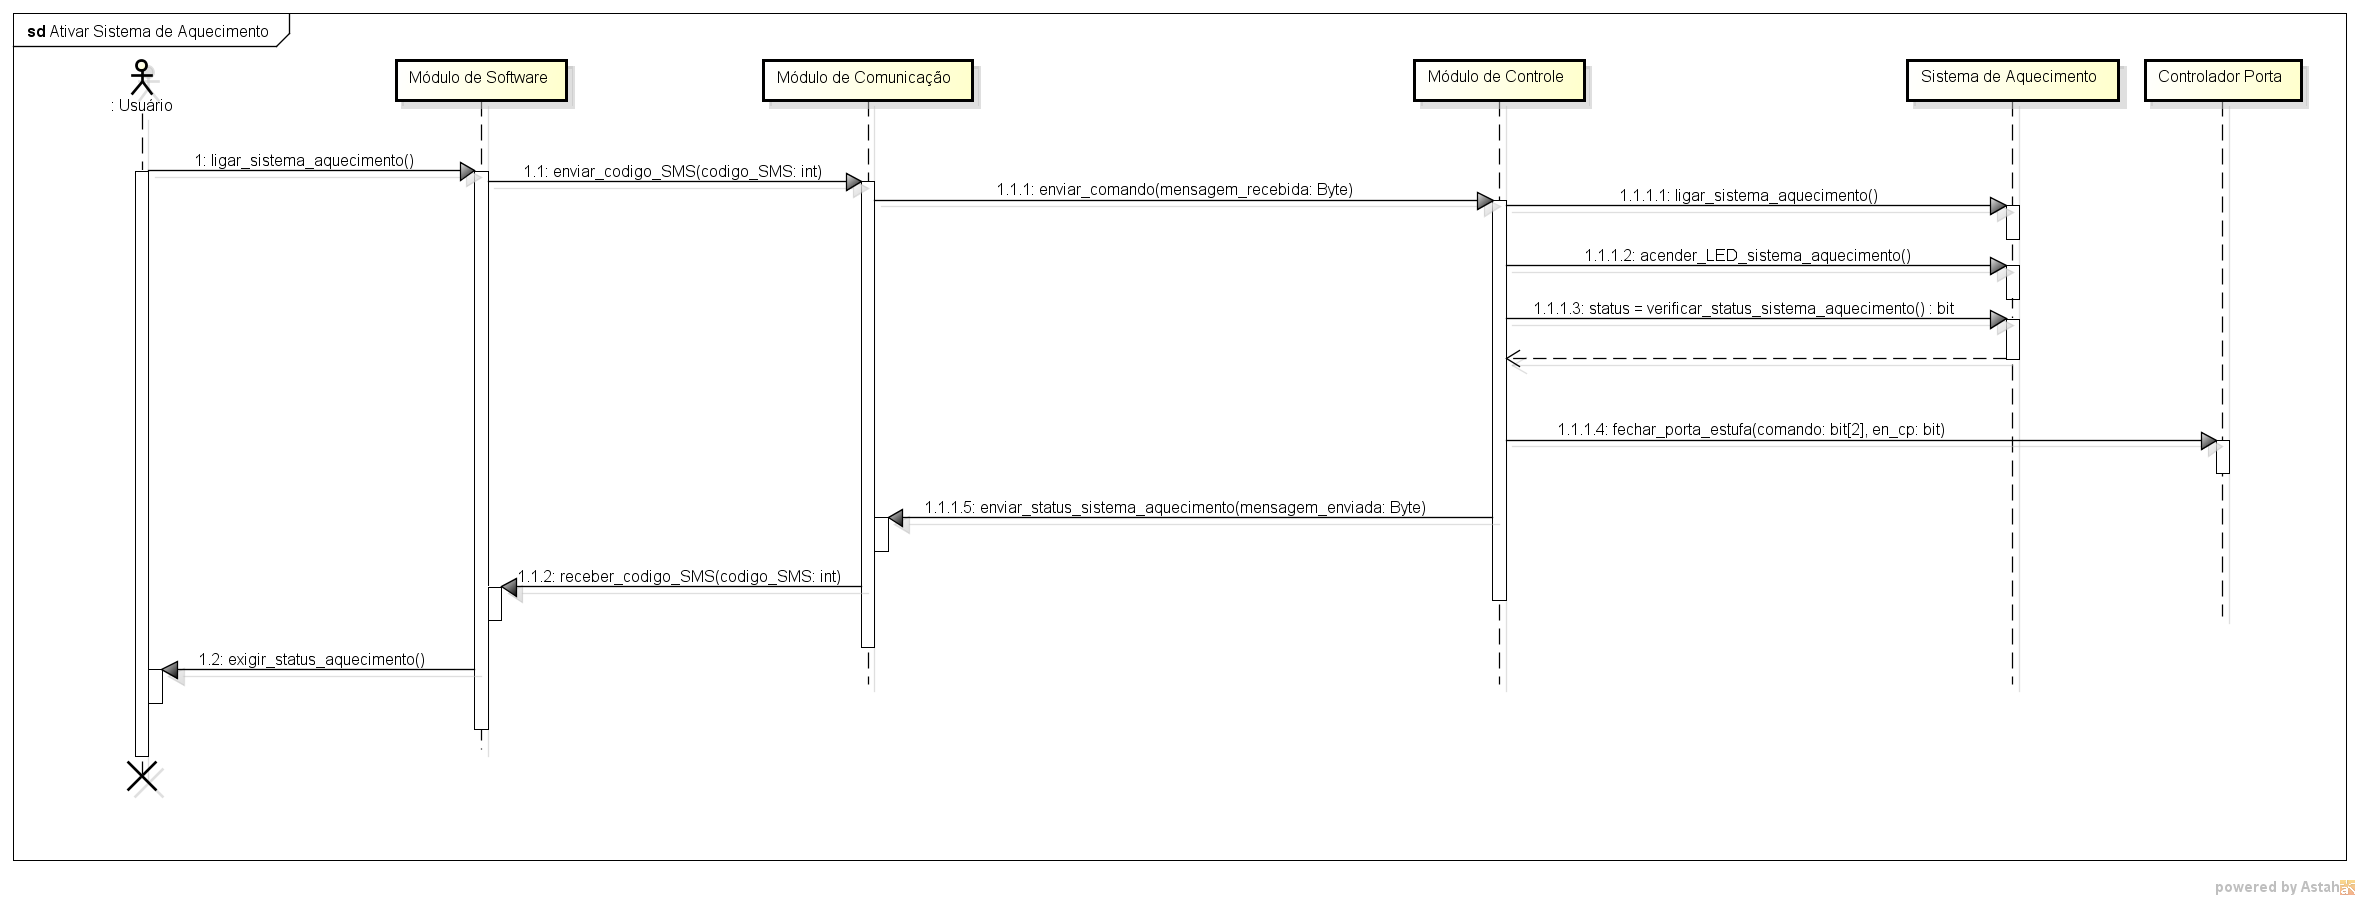
\includegraphics[width=\linewidth, height = 12cm]{pictures/ativar_sistema_aquecimento.png}
	      \caption{Diagrama de Atividade para acionamento do Sistema de Aquecimento da Estufa.}
	      \label{figure:ativar_sistema_aquecimento}
	     \end{figure}
	\end{landscape}
   
	\begin{landscape}
	    \begin{figure}[H]
	      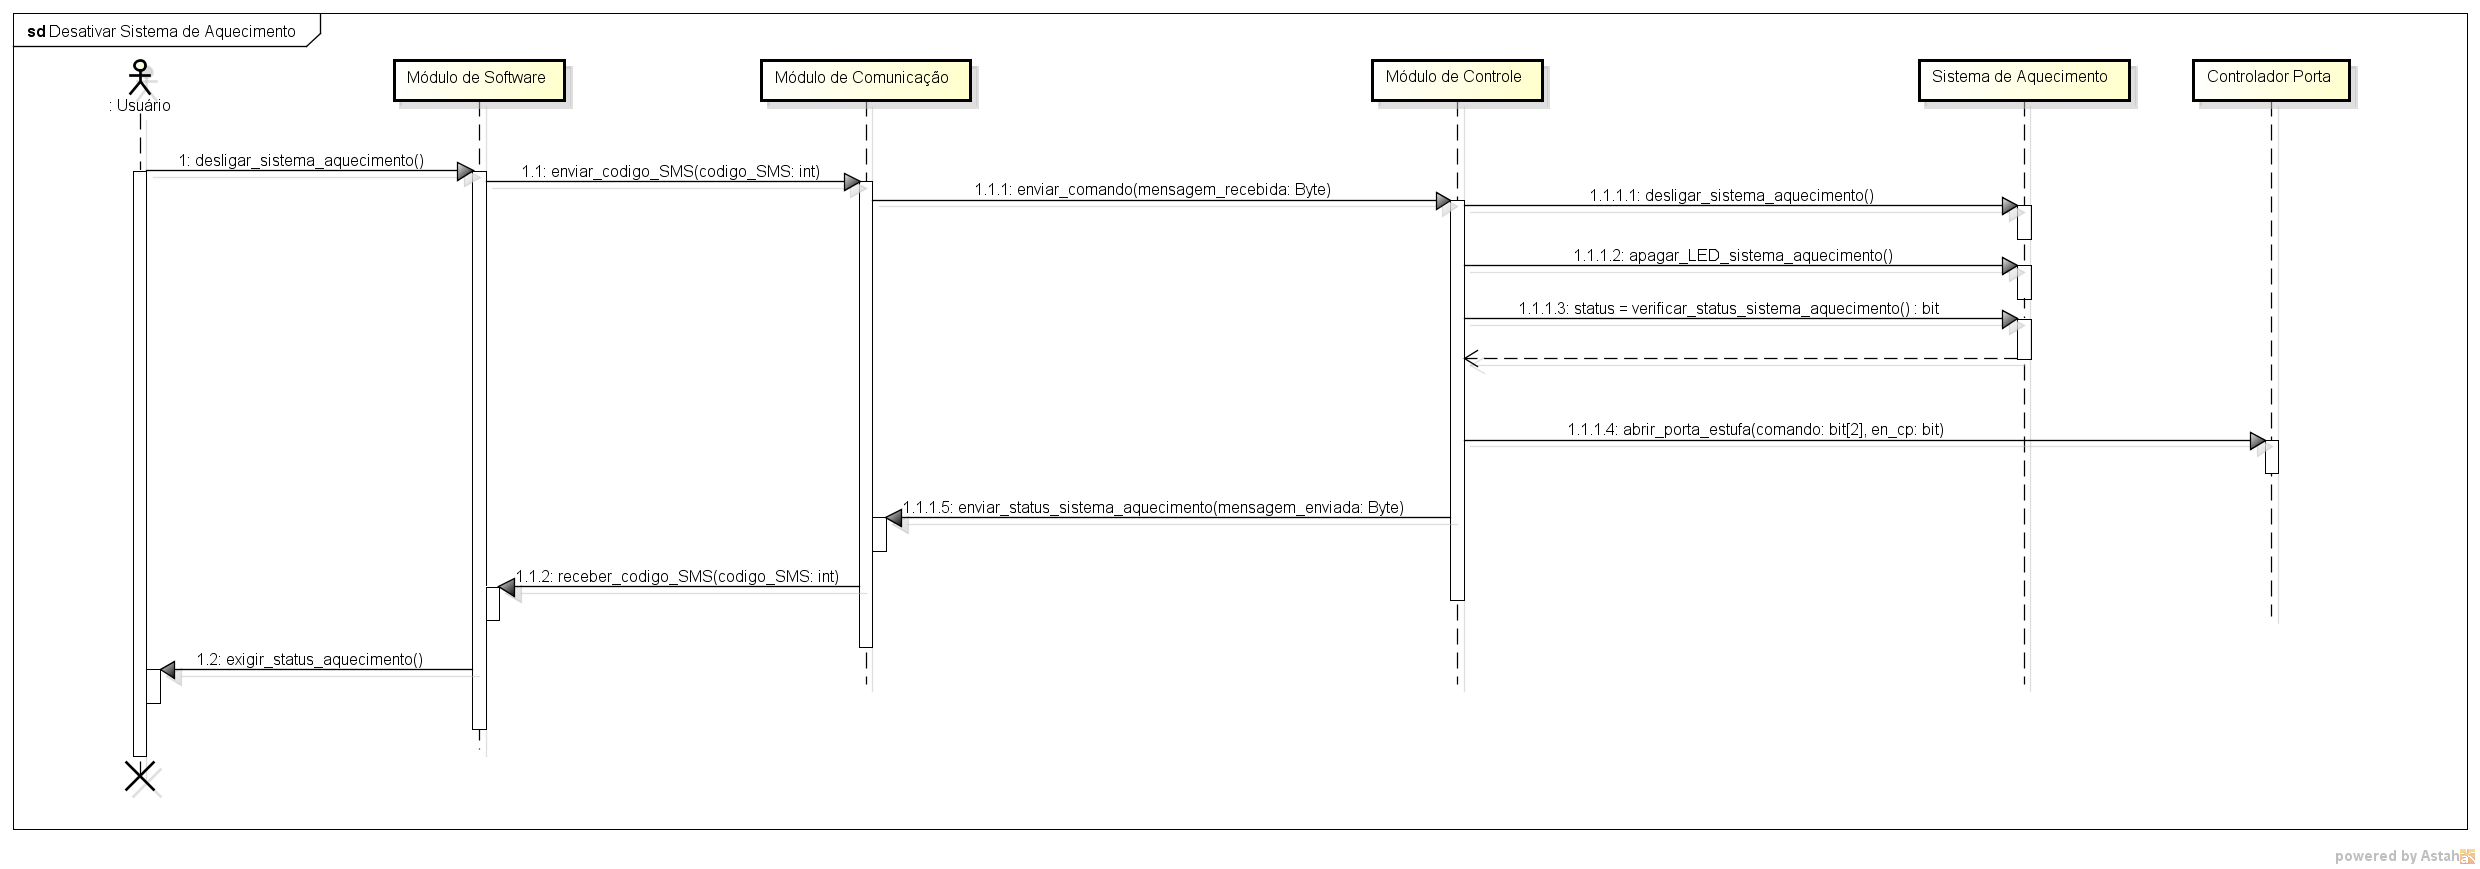
\includegraphics[width=\linewidth, height = 12cm]{pictures/desativar_aquecimento.png}
	      \caption{Diagrama de Atividade para desativar o Sistema de Aquecimento da Estufa.}
	      \label{figure:desativar_aquecimento}
	      \end{figure}
	\end{landscape}
	\begin{landscape}
	      \begin{figure}[H]
		  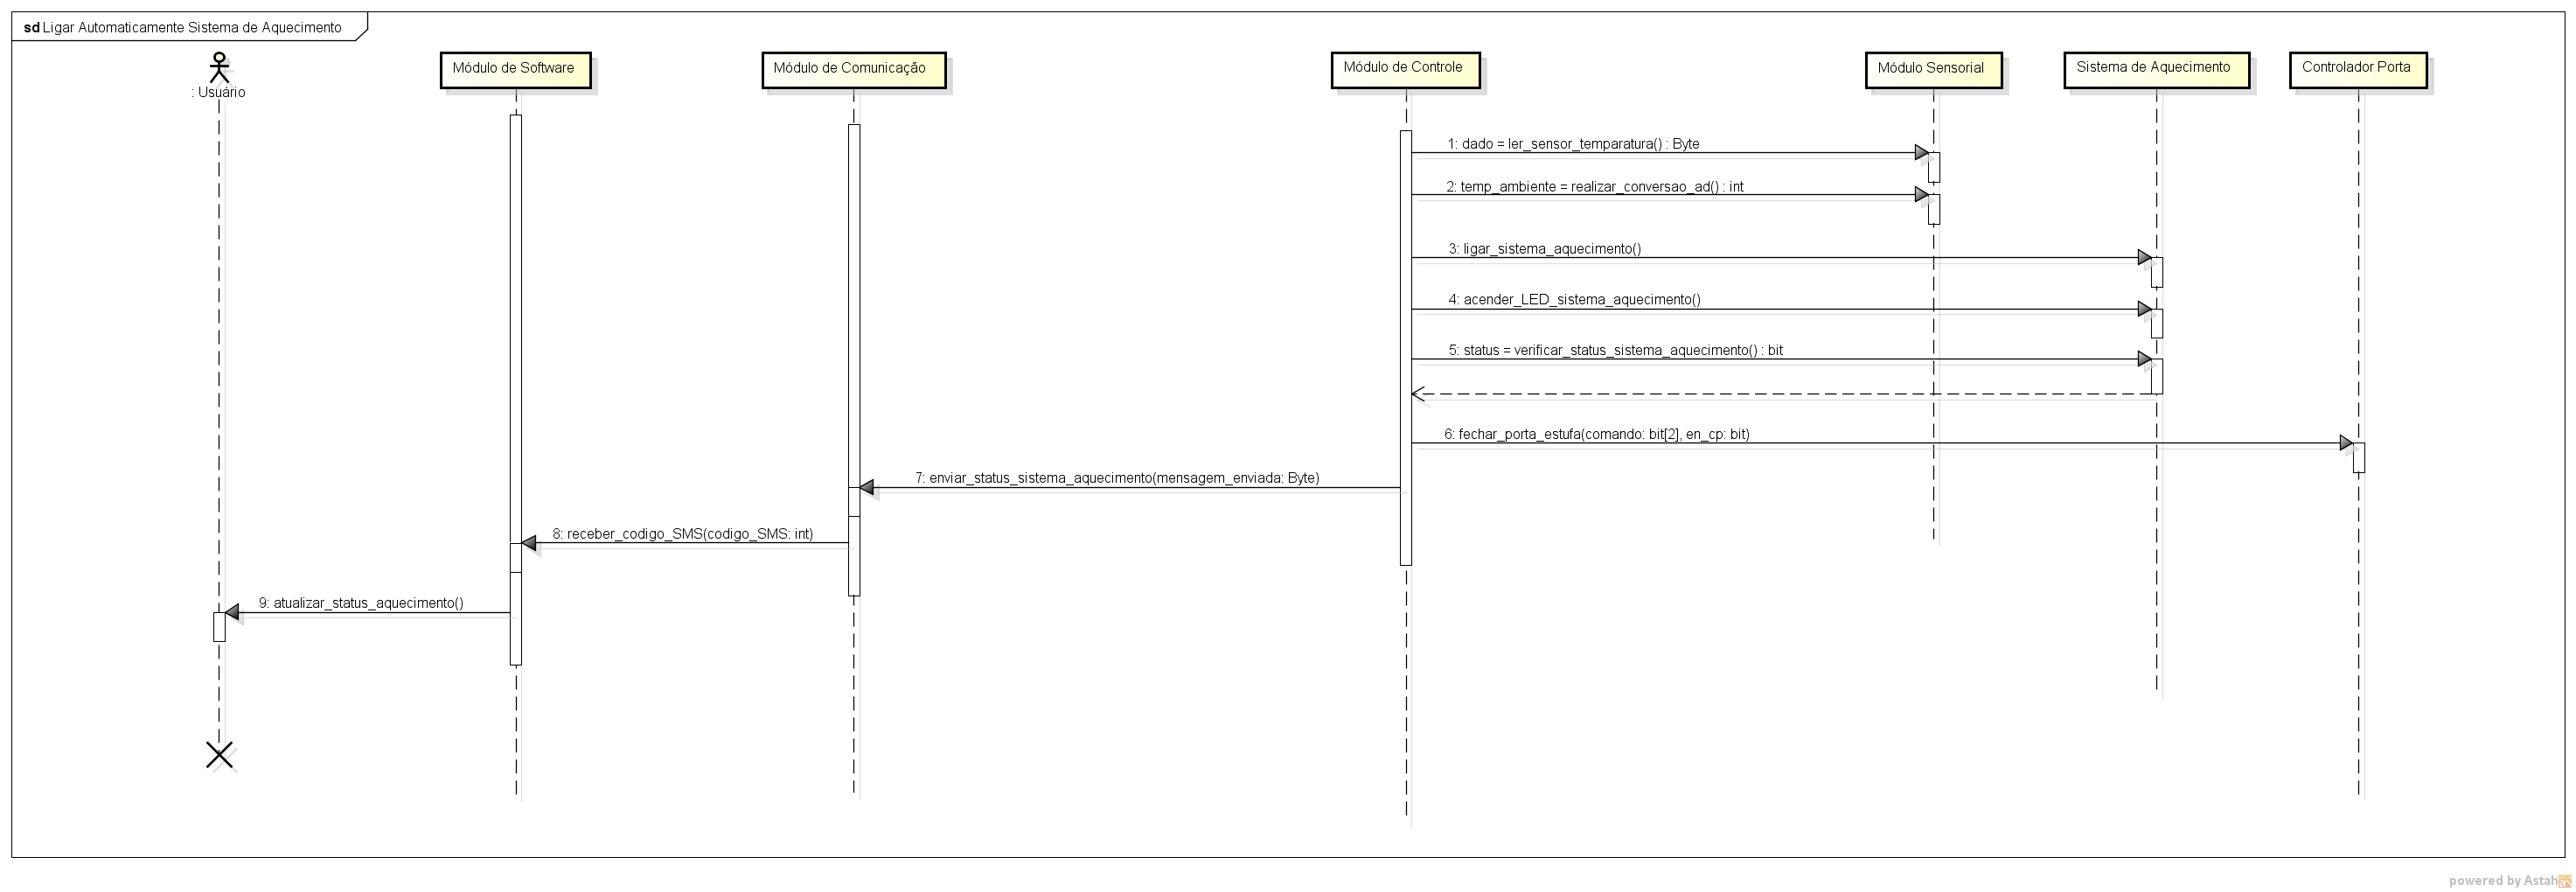
\includegraphics[width=\linewidth, height = 12cm]{pictures/ligar_automaticamente_sistema_aquecimento.png}
		  \caption{Diagrama de Atividade para acionamento automático do Sistema de Aquecimento da Estufa.}
		  \label{figure:ligar_automaticamente_sistema_aquecimento}
	      \end{figure}
	\end{landscape}
	
	\begin{landscape}
	    \begin{figure}[H]
		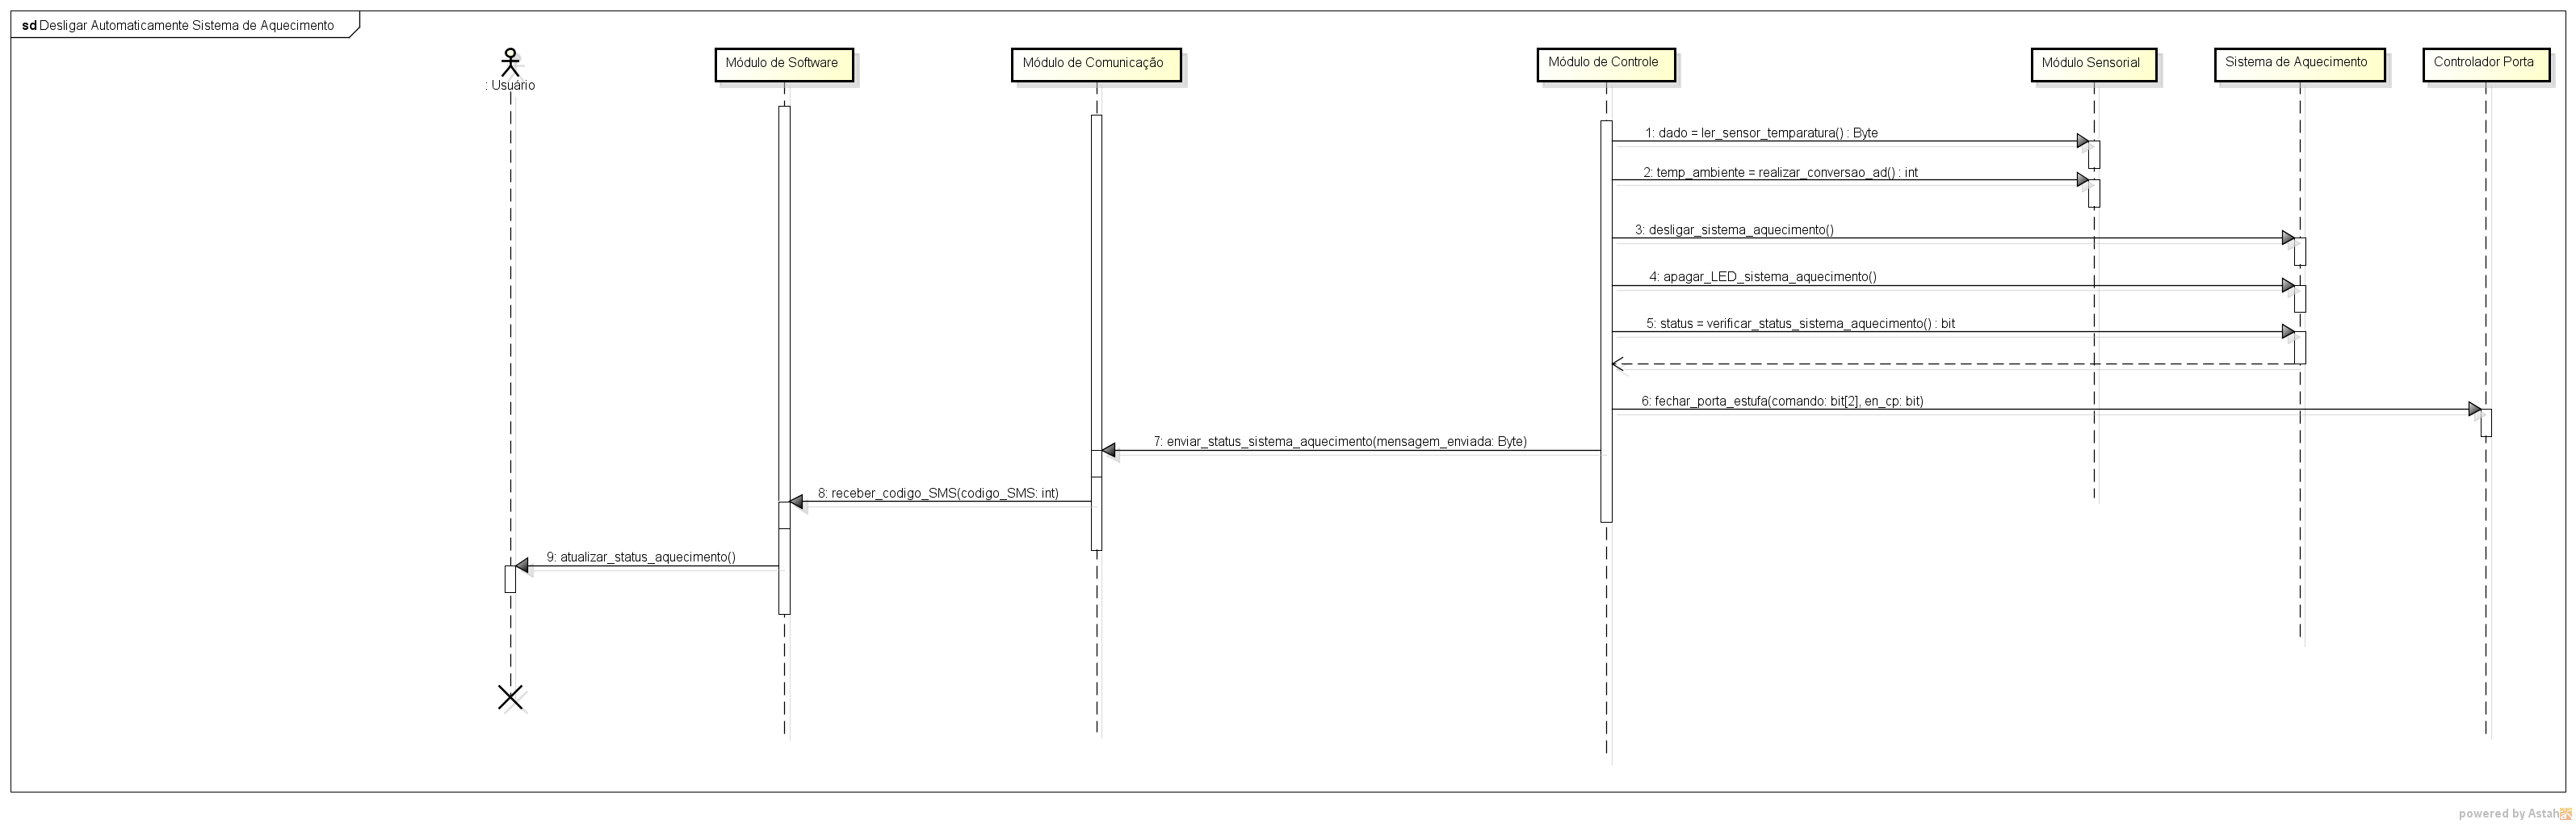
\includegraphics[width=\linewidth, height = 12cm]{pictures/desligar_automaticamente_aquecimento.png}
		\caption{Diagrama de Atividade para desativar automaticamente o Sistema de Aquecimento da Estufa.}
		\label{figure:desligar_automaticamente_aquecimento}
	    \end{figure}
	\end{landscape}
	
	
	\begin{landscape}
	    \begin{figure}[[H]
		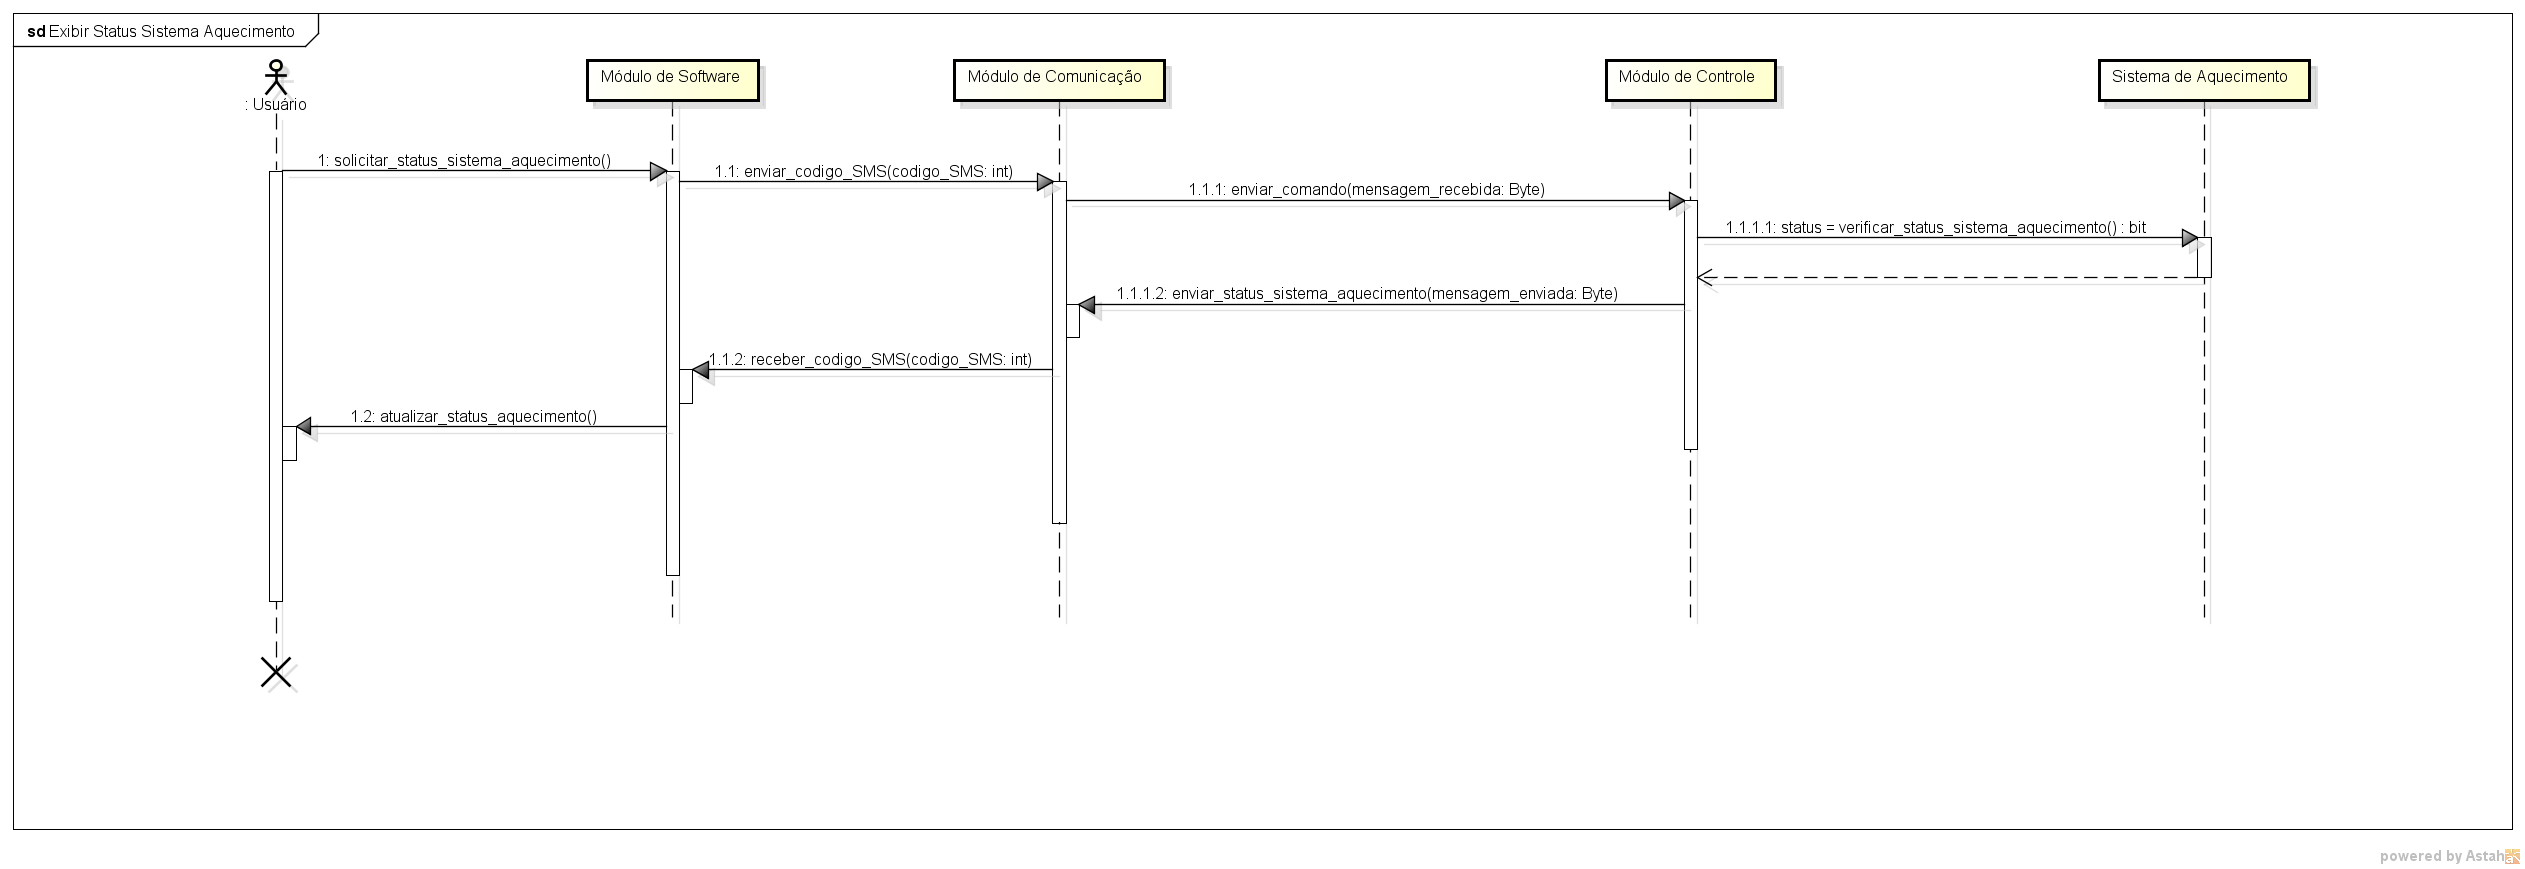
\includegraphics[width=\linewidth, height = 12cm]{pictures/status_sistema_aquecimento.png}
		\caption{Diagrama de Atividade para atualização do status do aquecimento da estufa a partir da aplicação Android.}
		\label{figure:status_sistema_aquecimento}
	    \end{figure}
	\end{landscape}
	
	
	\begin{landscape}
	    \begin{figure}[H]
		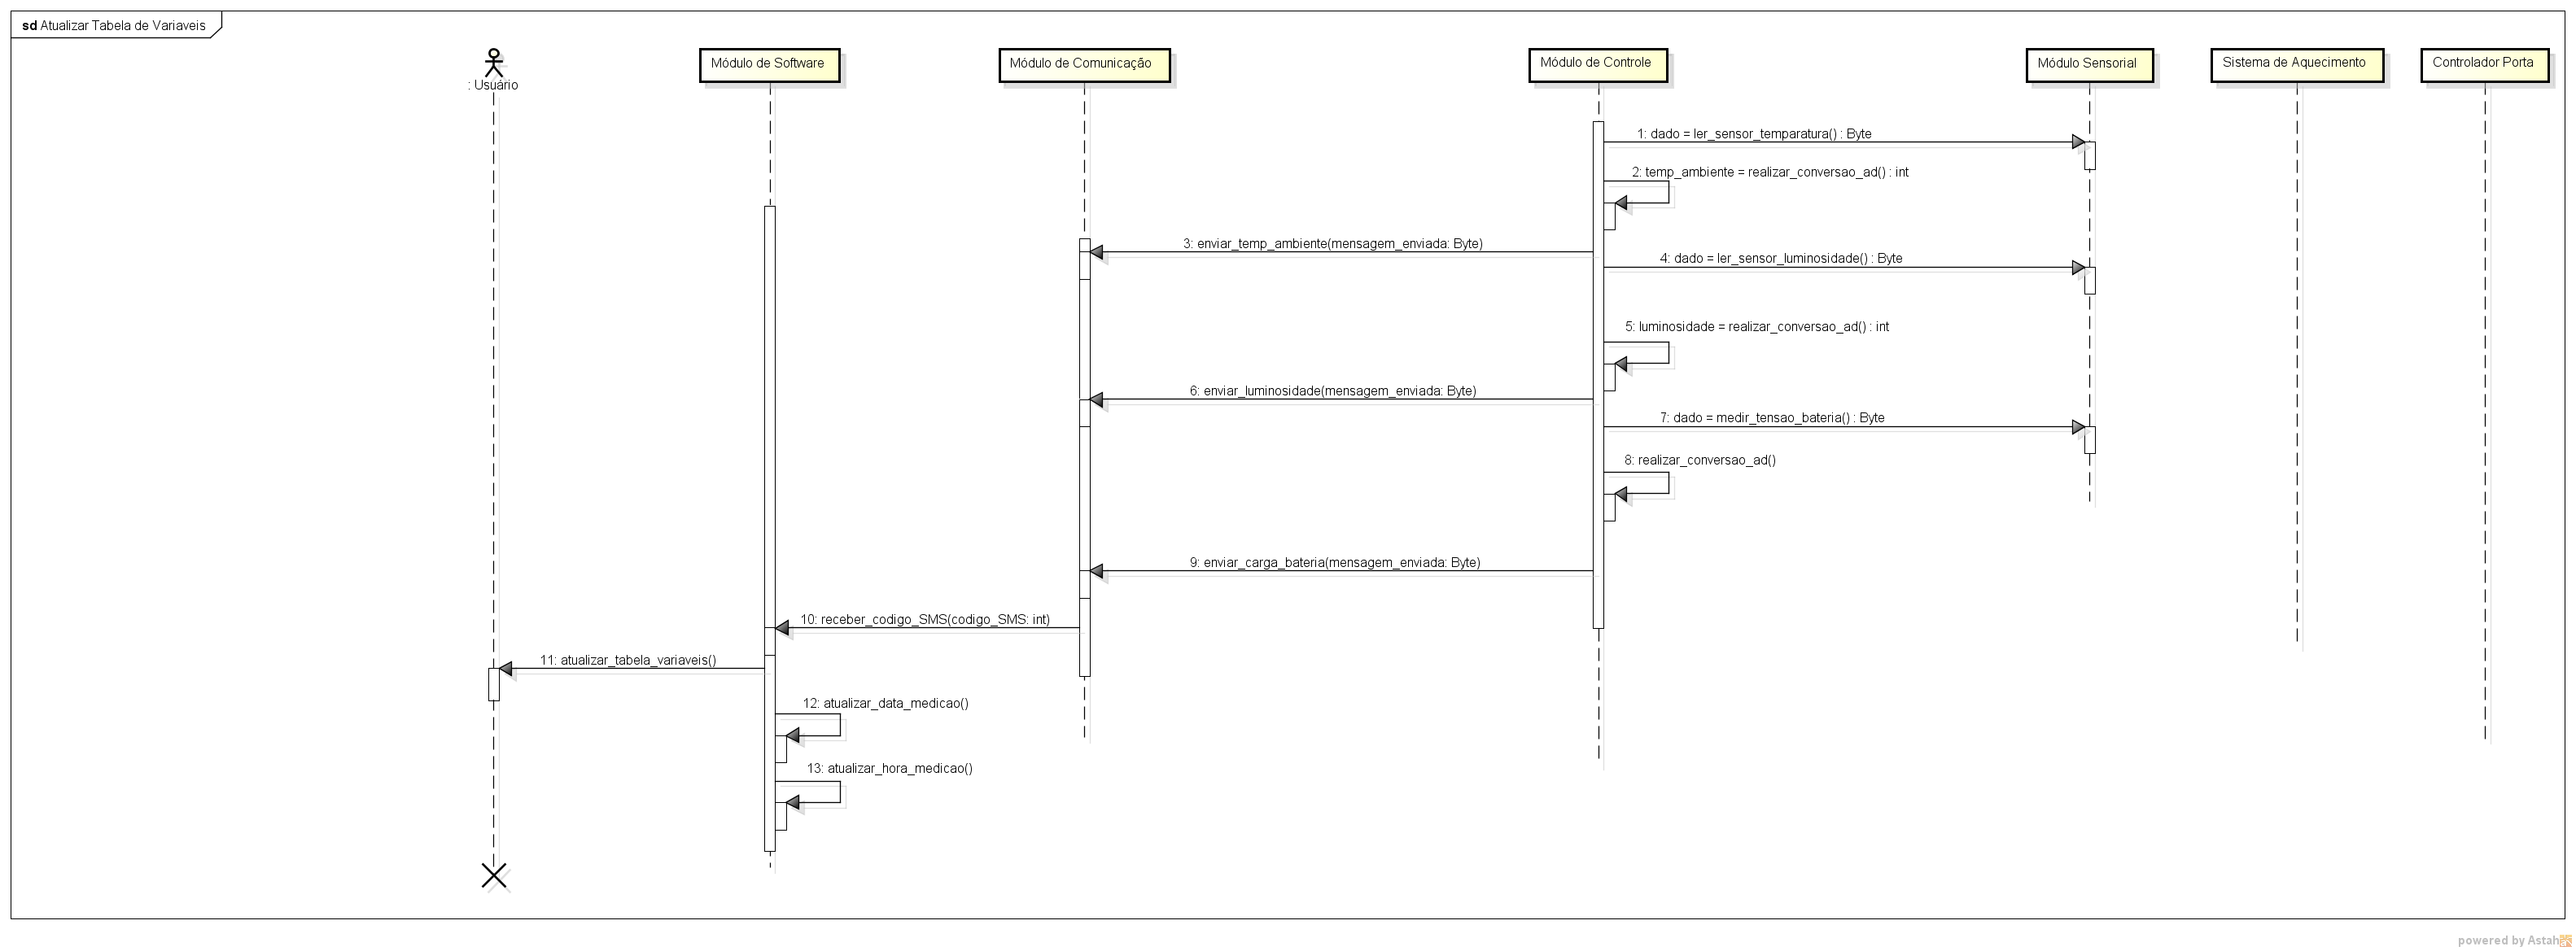
\includegraphics[width=\linewidth, height = 12cm]{pictures/atualizar_tabela_variaveis.png}
		\caption{Diagrama de Atividade para atualização dos dados da estufa a partir da aplicação Android.}
		\label{figure:atualizar_tabela_variaveis}
	    \end{figure}
	\end{landscape}
	
	
	
   \section{Diagrama de Estado}
  
      Os Diagramas de Estado apresentados nas Figuras {\ref{figure:sa_hw}}, {\ref{figure:sa_sw}}, {\ref{figure:troca_info}} apresentam 
      o comportamento e os eventos necessários para a mudança de estado do sistema. A Figura \ref{figure:sa_hw} apresenta o acionamento
      do sistema de aquecimento da estufa e as condições de eventos para cada estado acontecer. A Figura \ref{figure:sa_sw} apresenta o
      mesmo propósito da Figura \ref{figure:sa_hw}, entretanto para a comunicação a partir do módulo em software. A Figura \ref{figure:troca_info}
      ilustra os estados do sistema durante a troca de mensagens da aplicação Android e o módulo em Hardware. 
  
    \begin{figure}[H]
	 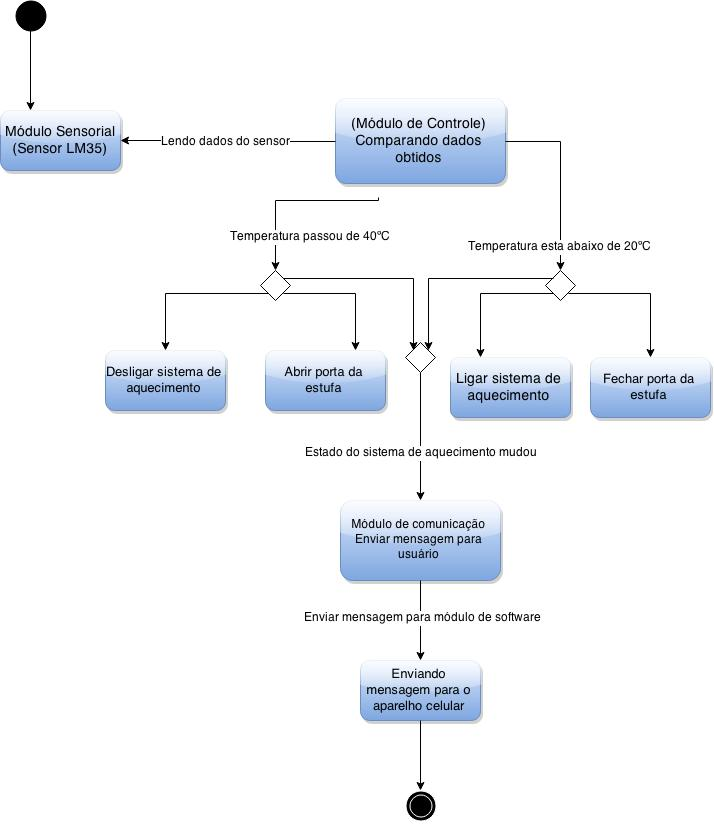
\includegraphics[width=\linewidth, height = 15cm]{pictures/sistema_aquecimento_estado.jpg}
	 \caption{Diagrama de Estado para o acionamento do Sistema de Aquecimento.}
	 \label{figure:sa_hw}
	\end{figure}
	
   \begin{figure}[H]
	 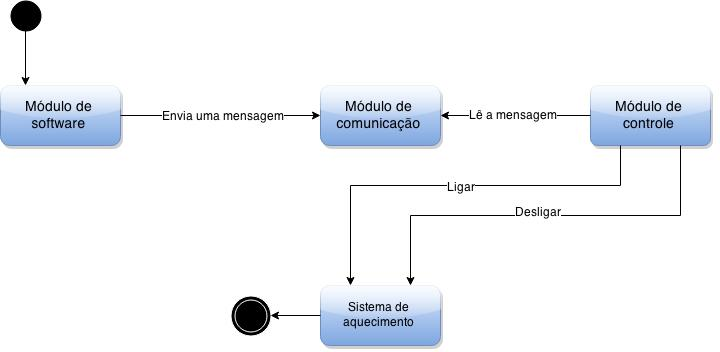
\includegraphics[height = 8cm, width = \linewidth]{pictures/sistema_aquecimento_estado_sw.jpg}
	 \caption{Diagrama de Estado para o acionamento do Sistema de Aquecimento via o aplicativo Android.}
	 \label{figure:sa_sw}
	\end{figure}
  
   \begin{figure}[H]
	 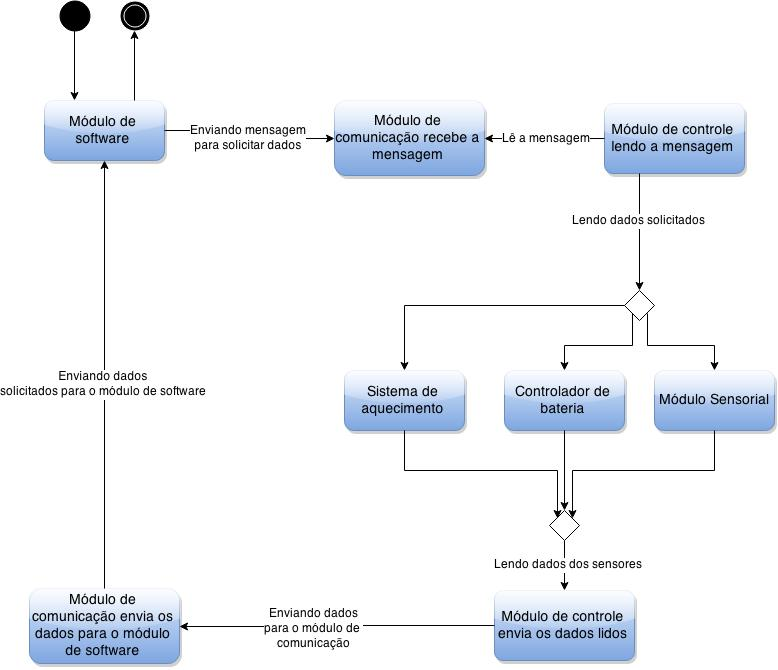
\includegraphics[width=\linewidth, height = 12cm]{pictures/troca_dados_estado.jpg}
	 \caption{Diagrama de Estado para troca de informações entre o Aplicativo Android e o módulo em Hardware.}
	 \label{figure:troca_info}
	\end{figure}

  
  \section{Ambiente de Desenvolvimento}
  
    Por se tratar de um sistema híbrido, o desenvolvimento do sistema aqui apresentado demanda dois tipos de ambientes de 
    desenvolvimento, um deles voltado para o aplicativo mobile e outro para o protótipo do sistema em hardware.
  
    O aplicativo mobile, a princípio exclusivo para o sistema Android, será desenvolvido utilizando o framework open-source SenchaTouch,
    que possibilita o desenvolvimento de aplicações híbridas utilizando tecnologias web como JavaScript, HTML5 e CSS3. O SenchaTouch implementa 
    o padrão arquitetural MVC (Model, View e Controller) além de possibilitar um processo de desenvolvimento ágil o que pode diminuir o tempo previsto
    para o desenvolvimento do aplicativo em comparação com o desenvolvimento de um aplicativo inteiramente nativo, por exemplo. O processo de
    desenvolvimento segue o mesmo de aplicações web, escrita de código em editor de texto e teste em browser. Uma grande vantagem oferecida
    por este framework é o fornecimento de recursos para exportar aplicativos de forma nativa, para outras plataformas além da Android, o que pode ser 
    útil para uma possível expansão do produto.


    O sistema em hardware contará com prototipação com auxílio do software Proteus, que garantirá a simulação do projeto antes de ser descarregado 
    no microcontrolador. O Proteus oferece um ambiente extremamente poderoso para simulação de circuitos incluindo a capacidade de simular adequadamente
    o funcionamento dos microcontroladores mais populares. As simulações realizadas neste software podem incluir instrumentos de medição que representam
    os sinais obtidos na simulação.


    O desenvolvimento do programa que será descarregado do microcontrolador será feito na MPLAB IDE (Integrated Development Environment), que é um ambiente
    de programação, simulação e gravação de microcontroladores. O MPLAB IDE é oferecido gratuitamente pela empresa Microchip Technology e foi escolhido por
    ter bom desempenho no desenvolvimento de aplicações e sistemas embarcados. Para descarregar o programa no microcontrolador será utilizado o PICKIT 2 que
    é uma ferramenta de gravação e debugação de microcontroladores PIC. Com o PICKIT 2 é possível fazer o debugger no próprio microcontrolador, além disso, 
    valores dos registradores do PIC podem ser enviados para o computador, possibilitando a análise dos valores na memória RAM e avaliação do desempenho do 
    programa.

% inicio das descrições de arquitetura para cada componente do sistema
\chapter{Descrição da Arquitetura de Hardware}

    \section{Introdução}
	Este capítulo tem por objetivo apresenta a arquitetura de Hardware de um sistema embarcado para controle de uma estufa. O 
	capítulo é subdividido em algumas seções, que descrevem a arquitetura mais detalhadamente. Na Seção {\ref{datapath}} é apresentado o 
	Datapath da arquitetura. Cada módulo no diagrama será representado por uma classe. Estas classes são apresentadas 
	nas Seções {\ref{mdComunicacao}}, {\ref{mdSensorial}}, {\ref{mdControlePorta}}, {\ref{mdAquecimento}} e {\ref{mdCentral}}.
	A Seção {\ref{esquema}}	ilustra o Esquema Elétrico Geral da arquitetura. 
      
      
    \section{Datapath}\label{datapath}
	
	O objetivo deste Datapath é apresentar a interconexão entre os módulos definidos para a arquitetura. A partir deste também é sabido o 
	relacionamento entre as classes de cada módulo descritos nas seções {\ref{mdComunicacao}}, {\ref{mdSensorial}}, {\ref{mdControlePorta}},
	{\ref{mdAquecimento}} e {\ref{mdCentral}}. A definição de componentes e funcionalidades podem ser visualizadas no Esquema Elétrico
	da Seção {\ref{esquema}}. 
	
     \section{Esquema Elétrico}\label{esquema}
    
	O Esquema Elétrico aqui apresentado objetiva dispor de uma visão mais específica sobre a implementação da arquitetura definida. Neste esquema é apresentado
	os componentes que serão utilizados e as interconexões entre estes. Como descrito na Seção {\ref{datapath}} o esquema apresenta as funcionalidades abstraídas 
	na Figura \ref{figure:datapath_geral}. 
    
	
      \begin{landscape}
	\begin{figure}[!h]
	  \begin{center}
	    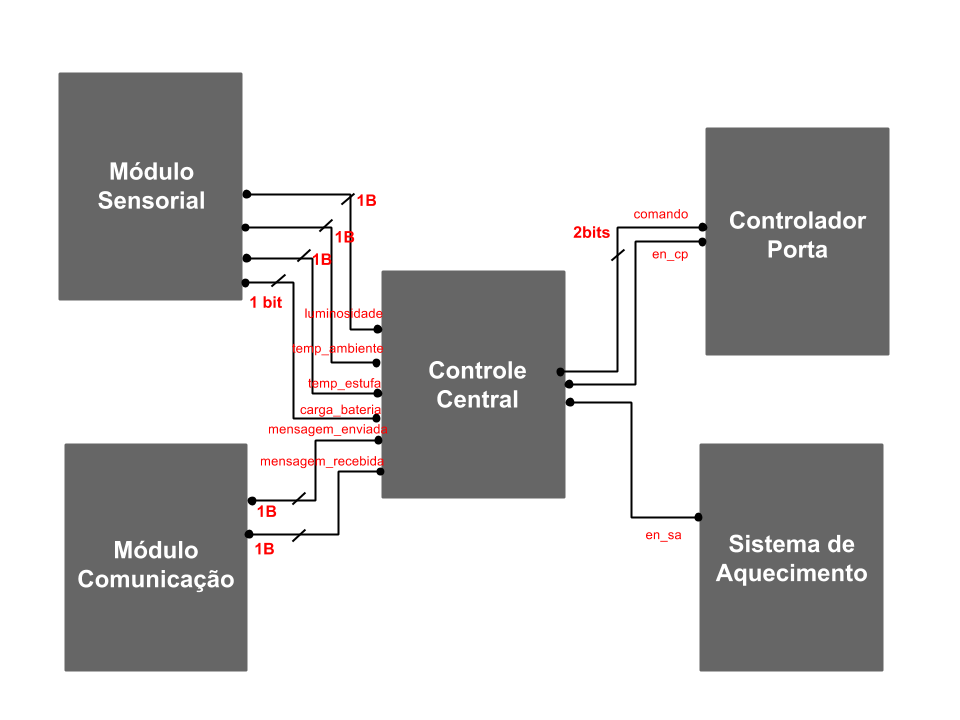
\includegraphics[width=\linewidth, height = 13cm]{pictures/data_path.png}
	    \caption{Datapath Geral da Arquitetura de Hardware.}
	    \label{figure:datapath_geral}
	  \end{center}
	\end{figure}
      \end{landscape}
   
      \begin{landscape}
	\begin{figure}[!h]
	    \begin{center}
	      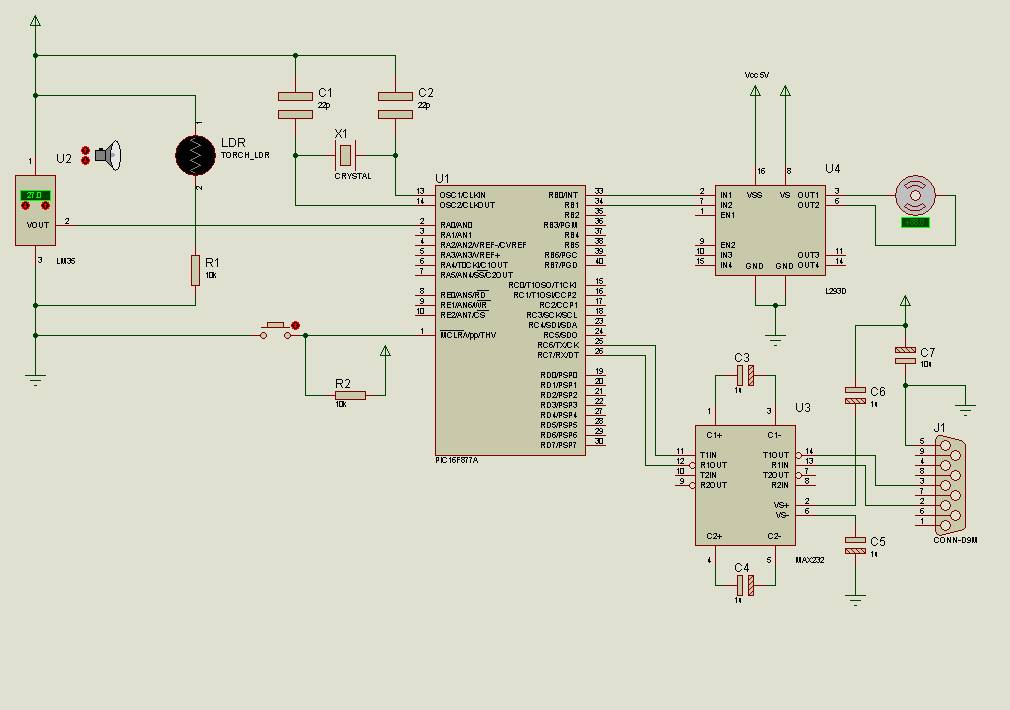
\includegraphics[width=\linewidth]{pictures/esquema.jpg}
	      \caption{Esquema Elétrico da arquitetura de Hardware.}
	  \end{center}
	\end{figure}
      \end{landscape}
      
    \section{Módulo de Comunicação}\label{mdComunicacao}
    
      \subsection{Descrição}
      
	  O módulo de comunicação é responsável por interligar a aplicação em software com o módulo de controle. Este módulo realiza a atividade de receber e enviar mensagens de 
	  textos. As mensagens recebidas devem ser enviadas ao módulo de controle que irá processar a informação. O módulo deve também receber uma mensagem do Controle Central e enviar
	  para o celular com a aplicação Android. Para realizar o envio e recepção das mensagens é utilizada um kit modem SIM 300 GSM-GPRS. O modem é conectado ao Controle Central 
	  a partir de uma conexão USART Síncrona. Os sinais transmitidos serão tratados a patir de um MAX 232 para serem adequados ao trabalho com o PIC (Controle Central). 
	  
      \subsection{Diagrama de Classe}
	\begin{figure}[H]
	  \centering
	  \begin{center}
	\begin{tikzpicture}
	\umlclass[type=class]{Modulo Comunicacao}{
	+ mensagem\_enviada : output bit [8] \\
	+ mensagem\_recebida : input bit [8] \\  }
	{- <<sequ>> enviar\_codigo\_SMS()\\
	 - <<sequ>> receber\_codigo\_SMS()\\
	 - <<sequ>> enviar\_comando()}
	\end{tikzpicture}
\end{center}
	\end{figure}
	
     \subsection{Definições de Entrada e Saída}
      \FloatBarrier
      \begin{center}
        \begin{longtable}[pos]{| l | c | c | m{7cm} |} \hline         
          \multicolumn{1}{|c|}{\cellcolor[gray]{0.9}\textbf{Nome}} & 
          \multicolumn{1}{c|}{\cellcolor[gray]{0.9}\textbf{Tamanho}} & 
          \multicolumn{1}{c|}{\cellcolor[gray]{0.9}\textbf{Direção}} &
          \multicolumn{1}{c|}{\cellcolor[gray]{0.9}\textbf{Descrição}} \\ \hline
          \endfirsthead
          \hline
          \multicolumn{4}{|l|}%
          {{\bfseries continuação da página anterior}} \\
          \hline
          \multicolumn{1}{|c|}{\cellcolor[gray]{0.9}\textbf{Nome}} & 
          \multicolumn{1}{c|}{\cellcolor[gray]{0.9}\textbf{Tamanho}} & 
          \multicolumn{1}{c|}{\cellcolor[gray]{0.9}\textbf{Direção}} &
          \multicolumn{1}{c|}{\cellcolor[gray]{0.9}\textbf{Descrição}} \\ \hline
          \endhead

          \multicolumn{4}{|r|}{{continua na próxima página}} \\ \hline
          \endfoot

          \hline
          \endlastfoot

          mensagem\_recebida   & 8   & entrada  & Mensagem de texto recebida pelo módulo de comunicação  \\ \hline
          mensagem\_enviada    & 8   & saída    & Mensagem de texto que deve ser enviada pelo módulo de comunicação    \\ 
        \end{longtable}
      \end{center}    

%%%%%%%%%%%%%%%%%%%%%%%%%%%%%%%%%%%%%%%%%%%%%%%%%%%

  \section{Módulo Sensorial}\label{mdSensorial}

      Este módulo tem o papel de concentrar o conjunto de sensores e o circuito medidor de carga. As informações são enviadas desses sensores para o Controle Central (PIC). 
      
    \subsection{Diagrama de Classe}
      \begin{figure}[H]
        \centering
        \begin{center}
	\begin{tikzpicture}
	\umlclass[type=class]{Modulo Sensorial}{
	+ temperatura\_estufa : output bit [10] \\
	+ temperatura\_ambiente : output bit [10] \\ 
	+ luminosidade\_ambiente : output bit [10] \\
	+ nivel\_bateria : output }
	{}
	\end{tikzpicture}
\end{center}
      \end{figure}

    \subsection{Definições de Entrada e Saída}
      \FloatBarrier
      \begin{center}
        \begin{longtable}[pos]{| l | c | c | m{7cm} |} \hline         
          \multicolumn{1}{|c|}{\cellcolor[gray]{0.9}\textbf{Nome}} & 
          \multicolumn{1}{c|}{\cellcolor[gray]{0.9}\textbf{Tamanho}} & 
          \multicolumn{1}{c|}{\cellcolor[gray]{0.9}\textbf{Direção}} &
          \multicolumn{1}{c|}{\cellcolor[gray]{0.9}\textbf{Descrição}} \\ \hline
          \endfirsthead
          \hline
          \multicolumn{4}{|l|}%
          {{\bfseries continuação da página anterior}} \\
          \hline
          \multicolumn{1}{|c|}{\cellcolor[gray]{0.9}\textbf{Nome}} & 
          \multicolumn{1}{c|}{\cellcolor[gray]{0.9}\textbf{Tamanho}} & 
          \multicolumn{1}{c|}{\cellcolor[gray]{0.9}\textbf{Direção}} &
          \multicolumn{1}{c|}{\cellcolor[gray]{0.9}\textbf{Descrição}} \\ \hline
          \endhead

          \multicolumn{4}{|r|}{{continua na próxima página}} \\ \hline
          \endfoot

          \hline
          \endlastfoot

          temperatura\_estufa     & 10  & saída  & Temperatura da estufa    \\ \hline
          temperatura\_ambiente   & 10  & saída  & Temperatura do ambiente \\ \hline 
          luminosidade\_ambiente  & 10  & saída  & Intensidade de luminosidade do ambiente \\ \hline 
          nivel\_bateria          & 1    & saída  & Nível da bateria solar: acima ou abaixo da metade. Deve ser utilizado 0 para abaixo e 1 para acima da metade. 
        \end{longtable}
      \end{center}    

    \section{Controle de Porta}\label{mdControlePorta}
      \subsection{Descrição}
	  Este módulo tem por objetivo controlar o motor de corrente contínua responsável por abrir ou fechar a porta da estufa. Para realizar esta atividade é utilizado
	  um CI L293D que implementa dois circuitos Ponte H. Para este fim somente é utilizado uma Ponte H. A partir dos valores de comando e enable enviados para o módulo 
	  a rotação do motor é controlada. 
	  
      \subsection{Diagrama de Classe}
	\begin{figure}[H]
	  \centering
	  \begin{center}
	\begin{tikzpicture}
	\umlclass[type=class]{Controle Porta}{
	+ comando : input bit [2] \\
	+ en\_cp : input \\}
	{-<<circ>> controla\_porta()\\}
	\end{tikzpicture}
\end{center}
	\end{figure}
    
    \subsection{Definições de Entrada e Saída}
      \FloatBarrier
      \begin{center}
        \begin{longtable}[pos]{| l | c | c | m{7cm} |} \hline         
          \multicolumn{1}{|c|}{\cellcolor[gray]{0.9}\textbf{Nome}} & 
          \multicolumn{1}{c|}{\cellcolor[gray]{0.9}\textbf{Tamanho}} & 
          \multicolumn{1}{c|}{\cellcolor[gray]{0.9}\textbf{Direção}} &
          \multicolumn{1}{c|}{\cellcolor[gray]{0.9}\textbf{Descrição}} \\ \hline
          \endfirsthead
          \hline
          \multicolumn{4}{|l|}%
          {{\bfseries continuação da página anterior}} \\
          \hline
          \multicolumn{1}{|c|}{\cellcolor[gray]{0.9}\textbf{Nome}} & 
          \multicolumn{1}{c|}{\cellcolor[gray]{0.9}\textbf{Tamanho}} & 
          \multicolumn{1}{c|}{\cellcolor[gray]{0.9}\textbf{Direção}} &
          \multicolumn{1}{c|}{\cellcolor[gray]{0.9}\textbf{Descrição}} \\ \hline
          \endhead

          \multicolumn{4}{|r|}{{continua na próxima página}} \\ \hline
          \endfoot

          \hline
          \endlastfoot

          comando     & 2  & entrada  & Define o sentido de giro do motor de corrente contínua.  \\ \hline 
          en\_cp	      & 1  & entrada  & Habilita a operação do módulo para o controle do motor. 
        \end{longtable}
      \end{center}    
    
   \section{Sistema de Aquecimento}\label{mdAquecimento}
   
   \subsection{Descrição}
      Sistema idependente que aquece a estufa quando ativado. O módulo de Controle Central apenas precisa ativá-lo quando solicitado, ou 
      quando a temperatura estiver fora do intervalo de 20 à 40 graus. 
   \subsection{Diagrama de Classe}
    \begin{figure}[H]
        \centering
        \begin{center}
	\begin{tikzpicture}
	\umlclass[type=class]{Sistema Aquecimento}{
	+ en\_sa : input bit \\
	}
	{}
	\end{tikzpicture}
\end{center}
      \end{figure}
   
   \subsection{Definições de Entrada e Saída}
     
     \FloatBarrier
      \begin{center}
        \begin{longtable}[pos]{| l | c | c | m{7cm} |} \hline         
          \multicolumn{1}{|c|}{\cellcolor[gray]{0.9}\textbf{Nome}} & 
          \multicolumn{1}{c|}{\cellcolor[gray]{0.9}\textbf{Tamanho}} & 
          \multicolumn{1}{c|}{\cellcolor[gray]{0.9}\textbf{Direção}} &
          \multicolumn{1}{c|}{\cellcolor[gray]{0.9}\textbf{Descrição}} \\ \hline
          \endfirsthead
          \hline
          \multicolumn{4}{|l|}%
          {{\bfseries continuação da página anterior}} \\
          \hline
          \multicolumn{1}{|c|}{\cellcolor[gray]{0.9}\textbf{Nome}} & 
          \multicolumn{1}{c|}{\cellcolor[gray]{0.9}\textbf{Tamanho}} & 
          \multicolumn{1}{c|}{\cellcolor[gray]{0.9}\textbf{Direção}} &
          \multicolumn{1}{c|}{\cellcolor[gray]{0.9}\textbf{Descrição}} \\ \hline
          \endhead

          \multicolumn{4}{|r|}{{continua na próxima página}} \\ \hline
          \endfoot

          \hline
          \endlastfoot
       
       en\_sa & 1  & entrada & Aciona o sistema de aquecimento. \\ \hline
       
       \end{longtable}
      \end{center}    
  
    \section{Controle Central}\label{mdCentral}

     \subsection{Descrição}
	  O Controle Central é o módulo responsável por processar as informações coletas no Módulo Sensorial e as mensagens enviadas pelo Módulo de Comunicação. Este módulo controla 
	  o acionamento do Sistema de Aquecimento e o Controle da Porta. O componente que representa este módulo é o PIC 16F877A. O PIC é responsável por converter os valores os dados, 
	  recebidos pelos sensores, em valores digitais, além de capturar as mensagens enviadas do módulo GPRS. Sua função é gerenciar, a depender da necessidade do usuário ou das 
	  variáveis do sistema, a temperatura da Estufa. 
	  
    \subsection{Diagrama de Classe}
	
	\begin{figure}[H]
	  \centering
	  \begin{center}
	\begin{tikzpicture}
	\umlclass[type=class]{Central Controle}{
	+ temperatura\_estufa : input bit [10] \\
	+ temperatura\_ambiente : input bit [10] \\ 
	+ luminosidade\_ambiente : input bit [10] \\
	+ nivel\_bateria : input \\
	+ mensagem\_recebida : input byte [8] \\
	+ mensagem\_enviada : output byte [8] \\ 
	+ en\_sa : output \\
	+ en\_cp : output \\
	+ comando : output bit[2] \\}
	{- <<comb>> ler\_sensor\_temperatura() \\
	- <<comb>> realizar\_conversao\_ad()\\
	- <<comb>> verificar\_status\_sistema\_aquecimento()\\
	- <<comb>> abrir\_porta\_estufa()
	- <<comb>> fechar\_porta\_estufa() \\
	- <<comb>> ligar\_sistema\_aquecimento()\\
	- <<comb>> desligar\_sistema\_aquecimento()\\
	- <<comb>> acender\_LED\_sistema\_aquecimento()\\
	- <<comb>> apagar\_LED\_sistema\_aquecimento()\\
	- <<sequ>> enviar\_status\_sistema\_aquecimento()\\
	- <<sequ>> enviar\_temp\_ambiente()\\
	- <<sequ>> enviar\_luminosidade()\\
	-<<sequ>> enviar\_carga\_bateria()\\  		
	}
	\end{tikzpicture}
\end{center}
	\end{figure}

	\subsection{Definições de Entrada e Saída}
	
	\FloatBarrier
	  \begin{center}
	  \begin{longtable}[pos]{| l | c | c | m{7cm} |} \hline         
	      \multicolumn{1}{|c|}{\cellcolor[gray]{0.9}\textbf{Nome}} & 
	      \multicolumn{1}{c|}{\cellcolor[gray]{0.9}\textbf{Tamanho}} & 
	      \multicolumn{1}{c|}{\cellcolor[gray]{0.9}\textbf{Direção}} &
	      \multicolumn{1}{c|}{\cellcolor[gray]{0.9}\textbf{Descrição}} \\ \hline
	      \endfirsthead
	      \hline
	      \multicolumn{4}{|l|}%
	      {{\bfseries continuação da página anterior}} \\
	      \hline
	      \multicolumn{1}{|c|}{\cellcolor[gray]{0.9}\textbf{Nome}} & 
	      \multicolumn{1}{c|}{\cellcolor[gray]{0.9}\textbf{Tamanho}} & 
	      \multicolumn{1}{c|}{\cellcolor[gray]{0.9}\textbf{Direção}} &
	      \multicolumn{1}{c|}{\cellcolor[gray]{0.9}\textbf{Descrição}} \\ \hline
	      \endhead
	      \multicolumn{4}{|r|}{{continua na próxima página}} \\ \hline
	      \endfoot
	      \hline
	      \endlastfoot

	      temperatura\_estufa     & 10  & entrada  & Temperatura da estufa    \\ \hline
	      temperatura\_ambiente   & 10  & entrada  & Temperatura do ambiente \\ \hline 
	      luminosidade\_ambiente  & 10  & entrada  & Intensidade de luminosidade do ambiente \\ \hline 
	      nivel\_bateria          & 1    & entrada & Nível da bateria solar: acima ou abaixo da metade \\ \hline 
	      mensagem\_recebida      & 8  & entrada   & Mensagem de texto enviada pelo módulo de comunicação. \\ \hline 
	      mensagem\_enviada       & 8  & saída    & Mensagem de texto a ser enviada pelo módulo de comunicação. \\ \hline 
	      en\_sa 		      & 1  & saída & Ativa o sistema de aquecimento da estufa \\ \hline 
	      en\_cp		      & 1  & saída & Ativa o controlador da porta \\ \hline
	      comando 		      & 2  & saída & Define a rotação do motor de corrente contínua. \\
	      
	  \end{longtable}
	  \end{center}    
  
\chapter{Descrição da Arquitetura de Software}
  
  \section{Introdução}
      Neste capítulo é apresentada a Arquitetura de Software desenvolvida. A aplicação será híbrida e contém um modelo de aplicação voltada a extrair, manipular e exibir para 
      o usuário (estruturado em uma tabela) as informações recebidas do outro módulo em Hardware. Essas informações são recebidas em mensagens de textos. A aplicação extraí o 
      conteúdo da mensagem e o manipula criando um DataInfo. Manipulando o objeto DataInfo é possível apresentar ao usuário as informações da Estufa. Além disso, são disponibilizadas
      as funções de ligar e desligar o Sistema de Aquecimento, assim como solicitar ou atualizar as informações. Na Seção {\ref{dmClasseSW}} é possível visualizar o Diagrama 
      de Classes da Aplicação Android. 
      
  \section{Diagrama de Classe}\label{dmClasseSW}

    \begin{landscape}
	\begin{figure}[H]
	    \begin{center}
	      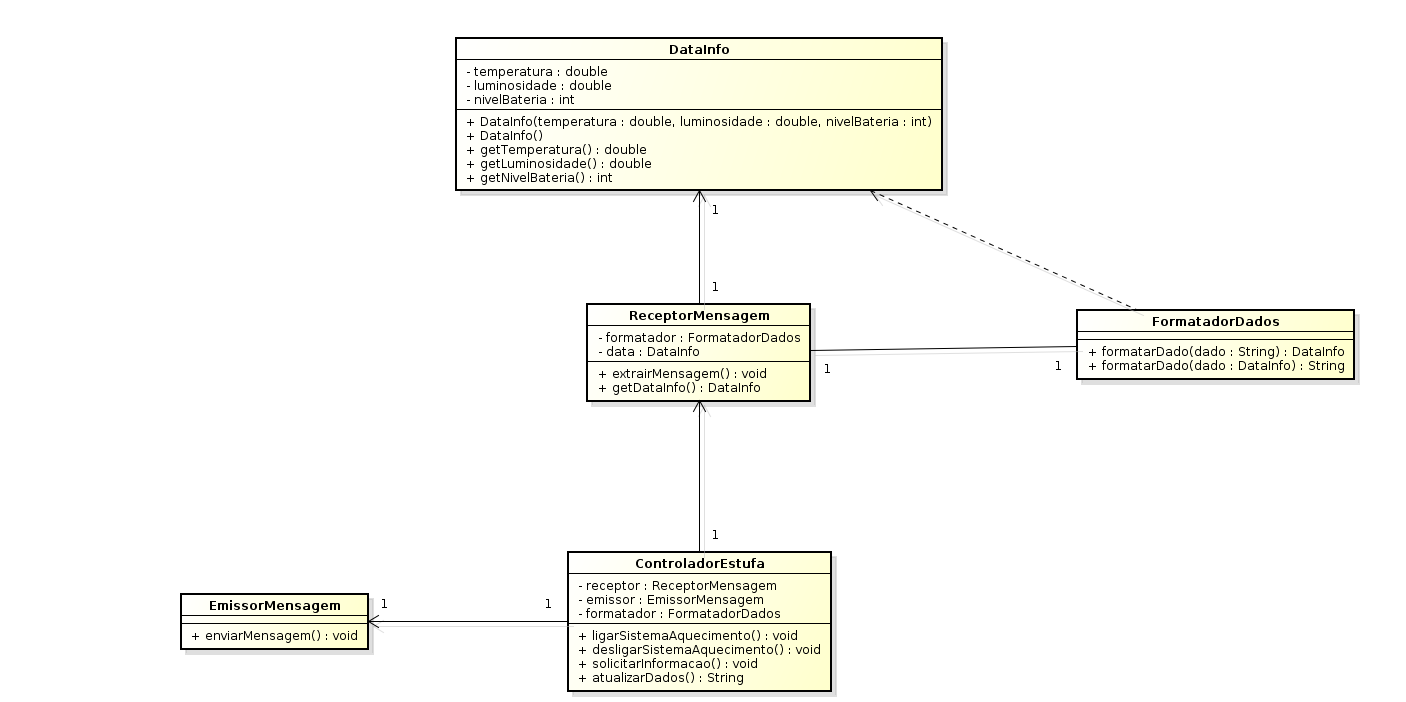
\includegraphics[width=\linewidth]{pictures/diagramaClassesSw.png}
	      \caption{Diagrama de Classes da Aplicação Android.}
	  \end{center}
	\end{figure}
    \end{landscape}

% Optional bibliography section
% To use bibliograpy, first provide the ipprocess.bib file on the root folder.
% \bibliographystyle{ieeetr}
% \bibliography{ipprocess}

\end{document}
